\begin{question}
\noindent Rectangle $ABCD$ is shown below.

\begin{center}
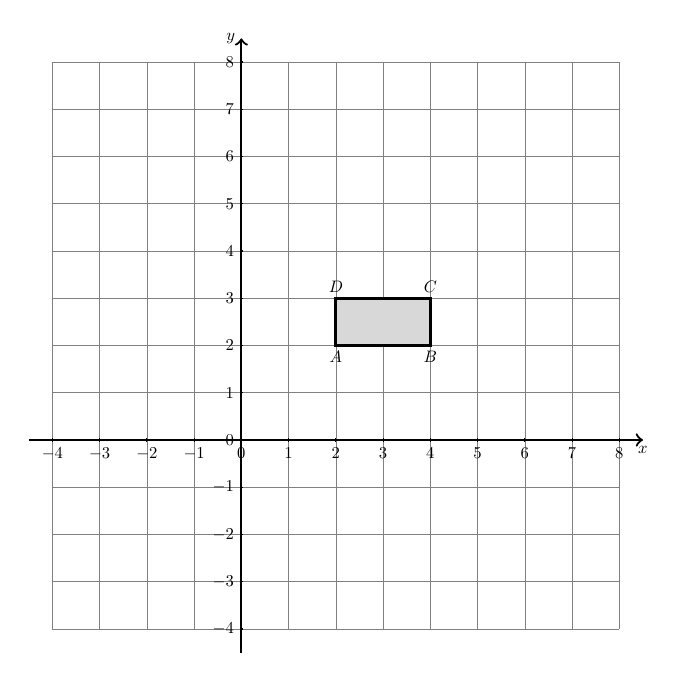
\begin{tikzpicture}[scale=0.6, transform shape]
    \definecolor{borderColour}{HTML}{000000}
    \definecolor{fillColour}{HTML}{D8D8D8}

    % Draw grid-Try and keep the grid even to avoid scaffolding or leading the student
    \draw[step=1cm,gray,very thin] (-4,-4) grid (8,8);

    % Draw axes
    \draw[thick,->] (-4.5,0) -- (8.5,0) node[anchor=north] {$x$};
    \draw[thick,->] (0,-4.5) -- (0,8.5) node[anchor=east] {$y$};

    % Label x-axis and y-axis
    \foreach \x in {-4,-3,-2,-1,...,8}
        \draw (\x cm,1pt) -- (\x cm,-1pt) node[anchor=north] {$\x$};
    \foreach \y in {-4,-3,-2,-1,...,8}
        \draw (1pt,\y cm) -- (-1pt,\y cm) node[anchor=east] {$\y$};

    % Original rectangle vertices
    \coordinate (A) at (2,2);
    \coordinate (B) at (4,2);
    \coordinate (C) at (4,3);
    \coordinate (D) at (2,3);

    \draw[fill=fillColour, draw=borderColour, line width=1pt] (A) -- (B) -- (C) -- (D) -- cycle;

    \node[below] at (A) {$A$};
    \node[below] at (B) {$B$};
    \node[above] at (C) {$C$};
    \node[above] at (D) {$D$};

\end{tikzpicture}
\end{center}

\noindent Enlarge rectangle $ABCD$ by scale factor $2$, centre $(1,1)$.

Work out the coordinates of the vertices of the image, $A'$, $B'$, $C'$ and $D'$.

\vspace{4cm}
\begin{flushright}
\answerplain{3}
\end{flushright}
\end{question}
